
\chapter{M\v{r}\'{\i}\v{z}kov\'{a} Boltzmannova metoda}
\label{chap:NumMet}

\pagestyle{plain}

    Numerick\'{a} metoda pou\v{z}it\'{a} k simulaci izoterm\'{a}ln\'{\i}ho proud\v{e}n\'{\i} tekutin je m\v{r}\'{\i}\v{z}kov\'{a} Boltzmannova metoda, zkr\'{a}cen\v{e} LBM. Tato metoda je jedna z nejmlad\v{s}\'{\i}ch hojn\v{e} pou\v{z}\'{\i}van\'{y}ch metod k simulaci tekutin. N\'{a}sleduj\'{\i}c\'{\i} kapitola se bude v\v{e}novat popisu t\'{e}to metody v prostoru $\mathbb{R}^3$.
    
    LBM pou\v{z}\'{\i}v\'{a} mezoskopick\'{e}ho popisu tekutiny, kdy uva\v{z}ujeme tekutinu slo\v{z}enou z \v{c}\'{a}stic a popsanou jedno\v{c}\'{a}sticovou pravd\v{e}podobnostn\'{\i} hustotou $f \ [\mathrm{kg \ m^{-6} \ s^{3}}]$. Funkce $f = f(\boldsymbol{x},\boldsymbol{\xi},t)$ zn\'{a}zor\v{n}uje pravd\v{e}podobnost, \v{z}e fiktivn\'{\i} \v{c}\'{a}stici najdeme v mal\'{e}m okol\'{\i}  ($H_{\boldsymbol{x}} \subset \mathbb{R}^3$) bodu $\boldsymbol{x}$, s rychlost\'{\i} v mal\'{e}m okol\'{\i} ($H_{\boldsymbol{\xi}} \subset \mathbb{R}^3$) rychlosti $\boldsymbol{\xi} = (\xi_1,\xi_2,\xi_3)^\intercal \ [\mathrm{m \ s^{-1}}]$ a v \v{c}ase $t \in \mathbb{R}^+_0$. Prostor rychlost\'{\i} budeme zna\v{c}it $\Xi $, tj. $\boldsymbol{\xi} \in \Xi = \mathbb{R}^3$. Takto zaveden\'{a} distribu\v{c}n\'{\i} funkce $f(\boldsymbol{x}, \boldsymbol{\xi},t)$ se pak \v{r}\'{\i}d\'{\i} Boltzmannovou transportn\'{\i} rovnic\'{\i}

    \begin{equation}
    \label{eq:BolTraEqu}
        \frac{\partial f}{\partial t} + \sum_{i=1}^{3}\xi_i \frac{\partial f}{\partial x_i} + \sum_{i=1}^{3}g_i \frac{\partial f}{\partial \xi_i} = \mathcal{C},
    \end{equation}
    kde $\boldsymbol{g} = (g_1, g_2, g_3)^T$ $[\mathrm{m \ s^{-2}}]$ vyjad\v{r}uje vektor zrychlen\'{\i} a $\mathcal{C} \  [\mathrm{kg \ m^{-6} \ s^{2}}]$ je kolizn\'{\i} oper\'{a}tor, kter\'{y} bude pops\'{a}n pozd\v{e}ji.
    
    \section{Diskretizace LBM}
    \label{sec:DisComDom}
        
        Diskretizace prostoru se v LBM prov\'{a}d\'{\i} za pomoci pravideln\'{e} m\v{r}\'{\i}\v{z}ky (angl. lattice). Diskretizace prostoru rychlost\'{\i} se potom odv\'{\i}j\'{\i} od zvolen\'{e}ho rychlostn\'{\i}ho modelu $DdQq$, kde $d$ a $q$ postupn\v{e} zna\v{c}\'{\i} dimenzi prostoru a po\v{c}et sm\v{e}r\r{u}, kter\'{y}mi se z ka\v{z}d\'{e}ho uzlu lze vydat. V t\'{e}to pr\'{a}ci budeme uva\v{z}ovat modely $D3Q27$ pro simulaci proud\v{e}n\'{\i} a $D3Q7$ pro \v{r}e\v{s}en\'{\i} advek\v{c}n\v{e}-difuzn\'{\i} rovnice. Oba modely jsou vyobrazeny na obr\'{a}zku \ref{fig:VelMod}. Modely maj\'{\i} n\'{a}sleduj\'{\i}c\'{\i} rozlo\v{z}en\'{\i} rychlost\'{\i}:

        \begin{itemize}
            \item[] D3Q27: \begin{align}
                \label{eq:VelModD3Q27}
                    \begin{split}            
                    \left\{\boldsymbol{\xi}_k\right\}_{k=0}^{26} = \vast\{ &\begin{pmatrix} 0 \\ 0 \\ 0 \end{pmatrix}, \begin{pmatrix} 1 \\ 0 \\ 0 \end{pmatrix}, \begin{pmatrix} 0 \\ 1 \\ 0 \end{pmatrix}, \begin{pmatrix} 0 \\ 0 \\ 1 \end{pmatrix}, \begin{pmatrix} -1 \\ 0 \\ 0 \end{pmatrix}, \begin{pmatrix} 0 \\ -1 \\ 0 \end{pmatrix}, \begin{pmatrix} 0 \\ 0 \\ -1 \end{pmatrix}, \begin{pmatrix} 0 \\ 1 \\ 1 \end{pmatrix}, \begin{pmatrix} 0 \\ 1 \\ -1 \end{pmatrix}, \begin{pmatrix} 0\\ -1 \\ 1 \end{pmatrix}, \begin{pmatrix} 0 \\ -1 \\ -1 \end{pmatrix},  \begin{pmatrix} 1 \\ 1 \\ 0 \end{pmatrix},  \begin{pmatrix} 1 \\ -1 \\ 0 \end{pmatrix}, \begin{pmatrix} -1 \\ 1 \\ 0 \end{pmatrix},  \\ 
                    &\begin{pmatrix} -1 \\ -1 \\ 0 \end{pmatrix}, \begin{pmatrix} 1 \\ 0 \\ 1 \end{pmatrix}, \begin{pmatrix} 1 \\ 0 \\ -1 \end{pmatrix}, \begin{pmatrix} -1 \\ 0 \\ 1 \end{pmatrix}, \begin{pmatrix} -1 \\ 0 \\ -1 \end{pmatrix}, \begin{pmatrix} 1 \\ 1 \\ 1 \end{pmatrix}, \begin{pmatrix} 1 \\ 1 \\ -1 \end{pmatrix}, \begin{pmatrix} 1 \\ -1 \\ 1 \end{pmatrix}, \begin{pmatrix} 1 \\ -1 \\ -1 \end{pmatrix}, \begin{pmatrix} -1 \\ 1 \\ 1 \end{pmatrix}, \begin{pmatrix} -1 \\ 1 \\ -1 \end{pmatrix}, \begin{pmatrix} -1 \\ -1 \\ 1 \end{pmatrix}, \begin{pmatrix} -1 \\ -1 \\ -1 \end{pmatrix} \vast\},
                    \end{split}
            \end{align}
            \item[] D3Q7: \begin{align}
                \label{eq:VelModD3Q7}
                    \left\{\boldsymbol{\xi}_k\right\}_{k=0}^{6} = \vast\{ &\begin{pmatrix} 0 \\ 0 \\ 0 \end{pmatrix}, \begin{pmatrix} 1 \\ 0 \\ 0 \end{pmatrix}, \begin{pmatrix} 0 \\ 1 \\ 0 \end{pmatrix}, \begin{pmatrix} 0 \\ 0 \\ 1 \end{pmatrix}, \begin{pmatrix} -1 \\ 0 \\ 0 \end{pmatrix}, \begin{pmatrix} 0 \\ -1 \\ 0 \end{pmatrix}, \begin{pmatrix} 0 \\ 0 \\ -1 \end{pmatrix} \vast\}.
                \end{align}
        \end{itemize}
        
        \begin{figure}[H]
            \centering
                \begin{subfigure}{.5\textwidth}
                    \centering
                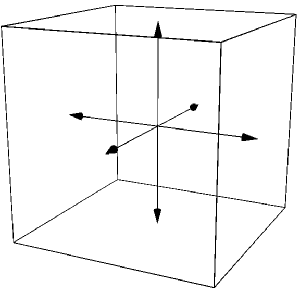
\includegraphics[width=.65\textwidth]{Img/Kapitola 2/D3Q7.pdf}
                \captionof{figure}{$D3Q7$.}
                \label{fig:VelMod2a}
                \end{subfigure}%
                \begin{subfigure}{.5\textwidth}
                \centering
                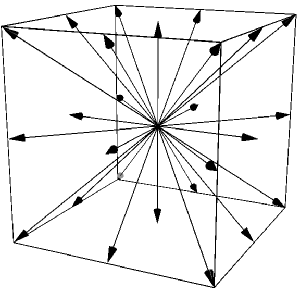
\includegraphics[width=.65\textwidth]{Img/Kapitola 2/D3Q27.pdf}
                \captionof{figure}{$D3Q27$.}
                \label{fig:VelMod2b}
                \end{subfigure}
                \caption{Zn\'{a}zorn\v{e}n\'{\i} rychlostn\'{\i}ch model\r{u} $D3Q7$ a $D3Q27$.}
                \label{fig:VelMod}
        \end{figure}

        V kapitole \ref{chap:MatMod} jsme definovali oblast $\Omega$, kterou nyn\'{\i} zdiskretizujeme izotropn\'{\i} m\v{r}\'{\i}\v{z}kou $\overline{\hat{\Omega}}$ ve tvaru
        \begin{subequations}
        \begin{align}
            \overline{\hat{\Omega}} &= \{ \boldsymbol{x}_{i,j,\ell} = \left(i h, j h, \ell h\right)^T \ | \ i \in \{0,1,...,N_{x}-1 \}, j \in \{0,1,...,N_{y}-1 \}, \ell \in \{0,1,...,N_{z}-1 \} \}, \label{eq:CloLatNod} \\
            \hat{\Omega} &= \{ \boldsymbol{x}_{i,j,\ell} \ | \ i \in \{1,2,...,N_{x}-2 \}, j \in \{1,2,...,N_{y}-2 \}, \ell \in \{1,2,...,N_{z}-2 \} \}, \label{eq:InnLatNod} \\
            \hat{\Gamma} &\coloneqq \overline{\hat{\Omega}} \backslash \hat{\Omega}, \label{eq:BorLatNod}
        \end{align}
        \end{subequations}
        kde $\hat{\Omega}$ zna\v{c}\'{\i} vnit\v{r}ek oblasti $\Omega$ a $\hat{\Gamma}$ ozna\v{c}uje uzly diskretizuj\'{\i}c\'{\i} hranici t\'{e}to oblasti. Prostorov\'{y} krok uva\v{z}ujeme ve v\v{s}ech sm\v{e}rech kart\'{e}zsk\'{y}ch os stejn\'{y} (tzv. ekvidistantn\'{\i} m\v{r}\'{\i}\v{z}ka), zna\v{c}me jej proto $h$. Diskretizovanou p\v{r}ek\'{a}\v{z}ku budeme zna\v{c}it $\overline{\hat{\Omega}_b} \subset \overline{\hat{\Omega}}$, jej\'{\i} hranic\'{\i} $\hat{\Gamma}_b$ budeme rozum\v{e}t uzly $\boldsymbol{x}_b \in \overline{\hat{\Omega}_b}$, pro kter\'{e} existuje $k \in \{ 1,2,...,q-1 \}$ takov\'{e}, \v{z}e m\v{r}\'{\i}\v{z}kov\'{y} bod $\boldsymbol{x}_b + \Delta t \boldsymbol{\xi}_k \notin \hat{\Omega}_b$.

        P\v{r}ed diskretizac\'{\i} samotn\'{e} Boltzmannovy rovnice zb\'{y}v\'{a} zav\'{e}st diskretizaci pro \v{c}asov\'{y} interval $\mathcal{I}$. Definujeme tedy diskr\'{e}tn\'{\i} interval 

        \begin{equation}
        \label{eq:DisTimInt}
                \hat{\mathcal{I}} = \{ t_i = i\Delta t \ | \ i \in \{ 0,1,...,N_{t}-1 \} \},
        \end{equation}
        ve kter\'{e}m $\Delta t = \frac{\mathcal{T}}{N_{t}}$ a $N_{t} \in \mathbb{N}$.
        
        % \begin{figure}[H]
        % \centering
        %     \begin{subfigure}[b]{0.8\textwidth}
        %        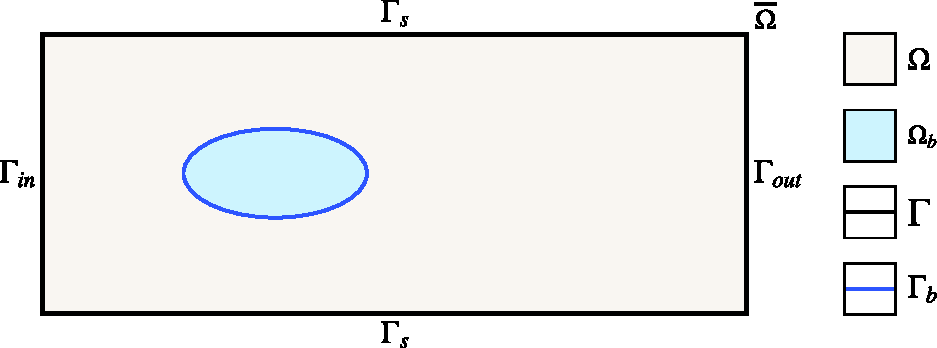
\includegraphics[width = \textwidth]{Img/Kapitola 2/domain2-1aa.pdf}
        %        \label{fig:Ng1} 
        %     \end{subfigure}
            
        %     \begin{subfigure}[b]{0.9\textwidth}
        %        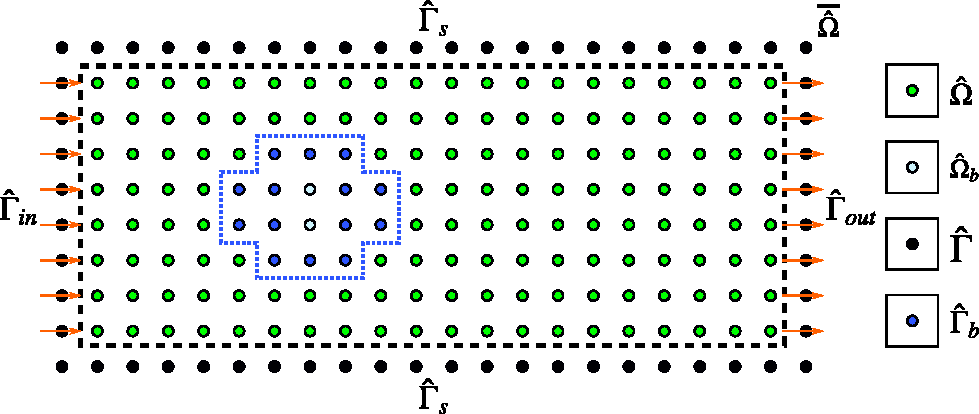
\includegraphics[width= \textwidth]{Img/Kapitola 2/domain2-1bb.pdf}              \caption{Dvourozm\v{e}rn\'{a} v\'{y}po\v{c}etn\'{\i} oblast $\Omega$ diskretizovan\'{a} ekvidistantn\'{\i} m\v{r}\'{\i}\v{z}kou $\overline{\hat{\Omega}}$ s diskr\'{e}tn\'{\i} hranic\'{\i} $\hat{\Gamma}$ rozd\v{e}lenou na vstup $\hat{\Gamma}_{in}$, st\v{e}ny $\hat{\Gamma}_s$ a odtokovou \v{c}\'{a}st $\hat{\Gamma}_{out}$.}
        %        \label{fig:Ng2}
        %     \end{subfigure}
            
        %     \caption{Sch\'{e}ma p\v{r}evodu dvourozm\v{e}rn\'{e} oblasti $\overline{\Omega}$ na diskr\'{e}tn\'{\i} oblast $\overline{\hat{\Omega}}$ pomoc\'{\i} izotropn\'{\i} ekvidistantn\'{\i} m\v{r}\'{\i}\v{z}ky. P\v{r}ek\'{a}\v{z}ka $\overline{\Omega}_b$ je diskretizovan\'{a} na $\overline{\hat{\Omega}}_b$ s hranic\'{\i} $\hat{\Gamma}_b$ a vnit\v{r}kem $\hat{\Omega}_b$.} 
        % \end{figure}
           
        Po zaveden\'{\i} diskretizace dost\'{a}v\'{a}me z \eqref{eq:BolTraEqu} diskr\'{e}tn\'{\i} Boltzmannovu transportn\'{\i} rovnici
        \begin{equation}
            \label{eq:DisBolTraEqu}
              f_k(\boldsymbol{x} + \Delta t \boldsymbol{\xi}_k, t + \Delta t) - f_k(\boldsymbol{x},t) = \mathcal{C}_k(\boldsymbol{x},t) + \mathcal{S}_k(\boldsymbol{x},t),
        \end{equation}
        kde $k \in \{ 0,1,2,...,q-1 \}$ je index sm\v{e}ru dan\'{e} rovnice v modelu $DdQq$. Na prav\'{e} stran\v{e} rovnice se vyskytuj\'{\i} kolizn\'{\i} oper\'{a}tor $\mathcal{C}_k$ a silov\'{y} \v{c}len $\mathcal{S}_k$, oba z\'{a}visl\'{e} na zvolen\'{e}m typu LBM \cite{kruger2017lattice, geier2015cumulant,guo2013lattice}. 

        P\v{r}i zaveden\'{\i} postkolizn\'{\i} distribu\v{c}n\'{\i} funkce $f_{k}^{*}$ vztahem
        \begin{equation}
            \label{eq:PosColFun}
                f_{k}^{*}(\boldsymbol{x},t) = f_{k}(\boldsymbol{x},t) + \mathcal{C}_k(\boldsymbol{x},t) + \mathcal{S}_k(\boldsymbol{x},t),
        \end{equation}
        m\r{u}\v{z}eme rovnici \eqref{eq:DisBolTraEqu} p\v{r}epsat do tvaru 
        \begin{equation}
            \label{eq:UpdDisBolEqu}    
                f_k(\boldsymbol{x} + \Delta t \boldsymbol{\xi}_k, t + \Delta t) = f_{k}^{*}(\boldsymbol{x},t),
        \end{equation}
        kter\'{y} plat\'{\i} $\forall \boldsymbol{x} \in \hat{\Omega}, \forall k \in \{ 0,1,...,q-1 \}, \forall t \in \{ 0,1,...,N_{t}-1 \}$.

        V r\'{a}mci kolizn\'{\i}ho kroku, kter\'{y} bude pops\'{a}n pozd\v{e}ji, se objevuje diskr\'{e}tn\'{\i} aproximace Maxwellovy-Boltzmannovy rovnov\'{a}\v{z}n\'{e} distribu\v{c}n\'{\i} funkce $f_{k}^{eq}$, $\forall k \in \{0,1,...,q-1 \}$. Ta je tvaru
        \begin{equation}
        \label{eq:EquDisFun}
            f_{k}^{eq}(\rho, \boldsymbol{u}) = \rho w_{k} \left( 1 + \frac{\boldsymbol{\xi}_{k} \cdot \boldsymbol{u}}{c_{s}^{2}} + \frac{(\boldsymbol{\xi}_{k} \cdot \boldsymbol{u})^{2}}{2c_{s}^{4}} - \frac{\boldsymbol{u} \cdot \boldsymbol{u}}{2c_{s}^{2}} \right).
        \end{equation}
        Hodnoty $c_s$ hraj\'{\i} roli m\v{r}\'{\i}\v{z}kov\'{e} rychlosti zvuku , kter\'{a} z\'{a}vis\'{\i} na zvolen\'{e}m modelu -- pro $D3Q27$ $c_s = \frac{1}{\sqrt{3}}$ a $c_s = \frac{1}{2}$ pro $D3Q7$. D\'{a}le se ve vztahu vyskytuj\'{\i} v\'{a}hy $w_k$, jejich\v{z} tvar je tak\'{e} ur\v{c}en rychlostn\'{\i}m modelem, kter\'{e}ho se dan\'{a} rovnov\'{a}\v{z}n\'{a} distribu\v{c}n\'{\i} funkce t\'{y}k\'{a} \cite{zou1995improved}. V\'{a}hy nab\'{y}vaj\'{\i} hodnot
        \begin{equation}
            \label{eq:VahyD3Q7}
                \left\{w_k\right\}_{k=0}^{6
                } = \left\{ \frac{1}{4}, \frac{1}{8}, \frac{1}{8}, \frac{1}{8}, \frac{1}{8}, \frac{1}{8}, \frac{1}{8} \right\} \qquad \mathrm{pro} \ D3Q7,
            \end{equation}
       a u modelu $D3Q27$ jsou to hodnoty
        \begin{equation}
            w_k = 
            \begin{cases} 
            \frac{8}{27}, & k = 0, \\ 
            \frac{2}{27}, & k \in \{ 1,2,3,...,6 \}, \\
            \frac{1}{54}, & k \in \{ 7,8,...,18 \}, \\
            \frac{1}{216}, & k \in \{ 19,20,...,26 \}.
            \end{cases} 
        \end{equation}
        


    
    \section{P\v{r}echod k bezrozm\v{e}rn\'{e}mu syst\'{e}mu jednotek}
    \label{sub:SysUni}    

        Pro zjednodu\v{s}en\'{\i} vzorc\r{u} pou\v{z}\'{\i}van\'{y}ch v LBM vol\'{\i}me m\v{r}\'{\i}\v{z}kov\'{y} prostorov\'{y} a \v{c}asov\'{y} krok dle \cite{kruger2017lattice} 
        \begin{equation}
            \Delta t = h = 1.
        \end{equation}    
        D\'{\i}ky t\'{e}to volb\v{e} pak z\'{\i}sk\'{a}v\'{a}me tyto p\v{r}evodn\'{\i} vztahy:
        \begin{subequations}
        \begin{align}
            \nu &= \frac{h^2}{\Delta t} \nu', \\
            D &= \frac{h^2}{\Delta t} D', \\
            u_i &= \frac{h}{\Delta t}u_i' \qquad \forall i \in \{1,2,3 \}, \\
            k &= \frac{h}{\Delta t}k',
        \end{align}
        \end{subequations}
        kde \v{c}\'{a}rkovan\'{e} veli\v{c}iny ozna\v{c}uj\'{\i} p\v{r}\'{\i}slu\v{s}n\'{e} veli\v{c}iny v m\v{r}\'{\i}\v{z}kov\'{y}ch jednotk\'{a}ch.  

        Hustota kapalin v LBM fluktuuje okolo sv\'{e} referen\v{c}n\'{\i} hodnoty $\rho_{ref}'$, kterou b\'{y}v\'{a} ve zvyku volit rovnu 1. V kapitole \ref{chap:MatMod} byl ale jedn\'{\i}m z p\v{r}edpoklad\r{u} na proud\v{e}n\'{\i} kapaliny jej\'{\i} nestla\v{c}itelnost. Z tohoto d\r{u}vodu b\'{y}v\'{a} LBM n\v{e}kdy ozna\v{c}ov\'{a}no za metodu \v{r}e\v{s}\'{\i}c\'{\i} slab\v{e} stla\v{c}iteln\'{e} proud\v{e}n\'{\i} \cite{kruger2017lattice}. Lze tedy ps\'{a}t 
        \begin{equation}
            \rho' = \rho_{ref}' + \delta_\rho'.
        \end{equation}




        

        % K \v{r}e\v{s}en\'{\i} neizoterm\'{a}ln\'{\i}ho proud\v{e}n\'{\i} (\'{u}loha \ref{sub:}) je nutn\'{e} prpojit jednotliv\'{e} modely LBM dohromady.

        % Cel\'{y} algoritmus m\v{r}\'{\i}\v{z}kov\'{e} Boltzmannovy metody lze rozd\v{e}lit do n\v{e}kolika \v{c}\'{a}st\'{\i}.
        
        % \begin{enumerate}
        %     \item \textbf{Inicializace}, b\v{e}hem kter\'{e} se nastav\'{\i} hodnoty diskr\'{e}tn\'{\i} distribu\v{c}n\'{\i} funkce podle po\v{c}\'{a}te\v{c}n\'{\i}ch a okrajov\'{y}ch podm\'{\i}nek. Oba typy podm\'{\i}nek budou pops\'{a}ny v sekci \ref{sec:BouIniCon}.
        %     \item \textbf{Cyklus} se bude opakovat, dokud nebude spln\v{e}na podm\'{\i}nka ukon\v{c}en\'{\i} simulace (dokud $t \le T$):
        %         \begin{enumerate}
        %             \item  V r\'{a}mci cyklu jsou nejprve \textbf{vypo\v{c}teny makroskopick\'{e} veli\v{c}iny} ze vztah\r{u} \eqref{eq:Mac}.
        %             \item N\'{a}sleduje \textbf{kolizn\'{\i} krok}, tj. vypo\v{c}\'{\i}taj\'{\i} se postkolizn\'{\i} distribu\v{c}n\'{\i} funkce pomoc\'{\i} vztahu \eqref{eq:UpdDisBolEqu}.
        %             \item P\v{r}i \textbf{kroku \v{s}\'{\i}\v{r}en\'{\i}} roze\v{s}le algoritmus hodnoty diskr\'{e}tn\'{\i}  distribu\v{c}n\'{\i} funkce v p\v{r}\'{\i}slu\v{s}n\'{y}ch sm\v{e}rech. N\'{a}sledn\v{e} se spo\v{c}tou hodnoty distribu\v{c}n\'{\i} funkce v dal\v{s}\'{\i}m \v{c}asov\'{e}m kroku. Ty z\'{a}vis\'{\i} pouze na hodnot\'{a}ch, kter\'{e} doraz\'{\i} z okoln\'{\i}ch uzl\r{u}.
        %             \item D\'{a}le nast\'{a}v\'{a} moment, kdy se \v{r}e\v{s}\'{\i} \textbf{okrajov\'{e} podm\'{\i}nky}. Ty pat\v{r}\'{\i} ke slo\v{z}it\v{e}j\v{s}\'{\i}m \v{c}\'{a}stem LBM, proto se jimi budeme v\v{e}novat v\'{\i}ce v n\'{a}sleduj\'{\i}c\'{\i} \v{c}\'{a}sti \ref{sec:BouIniCon}.
        %         \end{enumerate}
        %     \item \textbf{Ukon\v{c}en\'{\i} algoritmu}.
        % \end{enumerate}
        
        % \begin{figure}[H]
        %     \centering
        %     \includegraphics{Img/Kapitola 2/Algorithm.pdf}
        %     \caption{Sch\'{e}ma algoritmu LBM.}
        %     \label{fig:Alg}
        % \end{figure}
    \section{Numerick\'{e} sch\'{e}ma pro proud\v{e}n\'{\i} tekutiny}
    \label{sec:NumSchFluFlo}
            
        \todo[inline]{Rozepsat}

        Rovnice proud\v{e}n\'{\i} tekutin budeme \v{r}e\v{s}it modelem $D3Q27$, pro kter\'{y} m\'{a}me sadu distribu\v{c}n\'{\i}ch funkc\'{\i} ozna\v{c}enou 
        \begin{align}
            &\{ f_k(\boldsymbol{x}, t)\ | \ k \in \{0,1,2,\dots,26 \} \} & \forall (\boldsymbol{x}, t) \in \overline{\hat{\Omega}} \times \mathcal{\hat{I}} \label{eq:SetDisFunNSE}
        \end{align}
        Tyto distribu\v{c}n\'{\i} funkce $f_k$ jsou \v{r}\'{\i}zeny diskr\'{e}tn\'{\i} Boltzmannovou transportn\'{\i} ronvic\'{\i} \eqref{eq:DisBolTraEqu}, kde za diskr\'{e}tn\'{\i} kolizn\'{\i} oper\'{a}tor $\mathcal{C}_k$ vol\'{\i}me kumulantn\'{\i} LBM kolizn\'{\i} oper\'{a}tor (CuLBM), \cite{geier2015cumulant}.

        Makroskopick\'{e} veli\v{c}iny z\'{\i}sk\'{a}me ze vztah\r{u} 
        \begin{subequations}
        \label{eq:MacQuaForNSE}
            \begin{align}
                \rho & = \sum_{k=0}^{26}f_k, \\
                \rho \boldsymbol{u} & = \sum_{k=0}^{26}f_k \boldsymbol{\xi}_{k} + \frac{1}{2}\Delta t \boldsymbol{g}, \label{eq:MacMom}
            \end{align}
        \end{subequations}
        kde p\v{r}i \v{r}e\v{s}en\'{\i} NSR odpov\'{\i}d\'{a} nult\'{y} moment hustot\v{e} a prvn\'{\i} moment vektoru hybnosti. Rychlost z\'{\i}sk\'{a}me z rovnice pro hybnost vyd\v{e}len\'{\i}m p\v{r}edem spo\v{c}tenou hustotou.

        Z\'{a}kladem kumulantn\'{\i}ho kolizn\'{\i}ho oper\'{a}toru jsou relaxa\v{c}n\'{\i} \v{c}asy makroskopick\'{y}ch moment\r{u}, kter\'{e} jsou z\'{a}rove\v{n}  Galileovsky invariantn\'{\i} a statisticky nez\'{a}visl\'{e}. M\v{e}jme tedy rychlostn\'{\i} model $D3Q27$, pro kter\'{y} jsou obecn\'{e} a centr\'{a}ln\'{\i} momenty ve tvaru
        \begin{equation}
        \label{eq:RawMomCum}
            m_{\boldsymbol{\boldsymbol{\alpha}}} \coloneqq \sum_{k=0}^{26}f_k \xi_{k,1}^{\alpha_1}{\xi}_{k,2}^{\alpha_2}{\xi}_{k,3}^{\alpha_3},
        \end{equation}
        a
        \begin{equation}
        \label{eq:CenMomCum}
            k_{\boldsymbol{\boldsymbol{\alpha}}} \coloneqq \sum_{k=0}^{26}f_k ({\xi}_{k,1} - {u}_{1})^{\alpha_1}({\xi}_{k,2} - {u}_{2})^{\alpha_2}({\xi}_{k,3} - {u}_{3})^{\alpha_3}, 
        \end{equation}
        kde $\boldsymbol{\alpha} = (\alpha_1, \alpha_2, \alpha_3)^\intercal \in \mathbb{Z}^3$ a $\boldsymbol{u}$ zna\v{c}\'{\i} po \v{r}ad\v{e} multiindex a makroskopickou rychlost.

        Kolizn\'{\i} oper\'{a}tor je tvaru \cite{geier2015cumulant}
        \begin{equation}
            \label{eq:CumOpe}
                \mathcal{C}(\boldsymbol{f}(\boldsymbol{x},t)) = \boldsymbol{M}^{-1}\boldsymbol{G}^{-1}\left(\boldsymbol{N}^{-1}\boldsymbol{S}\boldsymbol{N}\boldsymbol{G}\Big(\boldsymbol{M}\boldsymbol{f}^{eq}(\boldsymbol{x},t) - \boldsymbol{M}\boldsymbol{f}(\boldsymbol{x},t)\Big)\right),
        \end{equation}
        tud\'{\i}\v{z} pro postkolizn\'{\i} distribu\v{c}n\'{\i} funkci dost\'{a}v\'{a}me vztah
        \begin{equation}
        \label{eq:PosColCum}
            \boldsymbol{f}^{*}(\boldsymbol{x},t) = \boldsymbol{f}(\boldsymbol{x},t) + \boldsymbol{M}^{-1}\boldsymbol{G}^{-1}\left(\boldsymbol{N}^{-1}\boldsymbol{S}\boldsymbol{N}\boldsymbol{G}\Big(\boldsymbol{M}\boldsymbol{f}^{eq}(\boldsymbol{x},t) - \boldsymbol{M}\boldsymbol{f}(\boldsymbol{x},t)\Big)\right),
        \end{equation}
        kde matice $\boldsymbol{S}$ je pro relaxa\v{c}n\'{\i} \v{c}asy $\tau_i, i \in \{ 0,1,\dots,26 \}$ ve tvaru
        \begin{equation}
        \label{eq:MatSCum}
            \boldsymbol{S} = \mathrm{diag}\Bigg(0, 0, 0, 0,  \frac{\Delta t}{\tau_1}, \frac{\Delta t}{\tau_2}, \frac{\Delta t}{\tau_3}, \frac{\Delta t}{\tau_4},\dots,\frac{\Delta t}{\tau_{22}}, \frac{\Delta t}{\tau_{23}} \Bigg).
        \end{equation}
        Pomoc\'{\i} matice $\boldsymbol{M}$ definujeme vektor makroskopick\'{y}ch moment\r{u} $\boldsymbol{\mu}$ jako
        \begin{equation}
            \label{eq:MatMCum}    
                \boldsymbol{\mu} = \boldsymbol{M}\boldsymbol{f}.
        \end{equation}
        Dal\v{s}\'{\i} matic\'{\i}, kter\'{a} vystupuje ve vztahu \eqref{eq:PosColCum}, je matice kombinace kumulant\r{u} $\boldsymbol{N}$. Podrobn\'{y} popis t\v{e}chto matic lze nal\'{e}zt v \cite{geier2015cumulant}. Posledn\'{\i}m v\'{y}razem, kter\'{y} vystupuje ve vztahu pro postkolizn\'{\i} funkce, je neline\'{a}rn\'{\i} oper\'{a}tor $\boldsymbol{G}$, za pomoci kter\'{e}ho je provedena transformace obecn\'{y}ch moment\r{u} $\boldsymbol{\mu}$ do kumulantn\'{\i}ho vektoru  
        \begin{equation}
            \label{eq:OpeGCum}
                \boldsymbol{\gamma} = \boldsymbol{G}(\boldsymbol{\mu}) = \boldsymbol{G(Mf)} = \left( \gamma_{(0,0,0)}, \gamma_{(1,0,0)}, \gamma_{(0,1,0)},\dots, \gamma_{(2,2,2)} \right)^\intercal.
        \end{equation}
        Nakonec definujeme vektor 
        \begin{equation}
            \label{eq:GamEquCum}
                \boldsymbol{\gamma}^{eq} = \left( \rho, 0, 0, 0, 0, 0, 0, 0, 0, 3\rho c_s^2, 0, 0,\dots,0 \right)^\intercal \in \mathbb{R}^{27}
        \end{equation}
        a n\'{a}sledn\v{e} m\r{u}\v{z}eme vztah \eqref{eq:PosColCum} p\v{r}epsat v \v{r}e\v{c}i vektoru $\boldsymbol{\gamma}$
        \begin{equation}
            \label{eq:PosColCumGam}
                \boldsymbol{\gamma}^* (\boldsymbol{x},t) = \boldsymbol{\gamma} (\boldsymbol{x},t) + \boldsymbol{N}^{-1}\boldsymbol{S}\boldsymbol{N} \Big( \boldsymbol{\gamma}^{eq} (\boldsymbol{x},t) - \boldsymbol{\gamma} (\boldsymbol{x},t)\Big).
        \end{equation}

        P\v{r}edpokl\'{a}d\'{a}me-li izotropn\'{\i} viskozitu, lze volit relaxa\v{c}n\'{\i} \v{c}asy 
        \begin{subequations}
            \begin{align}
                \tau_1 &= \tau_{shear}, \\
                \tau_i &= 1  \qquad \forall i \in \{ 2,3,4,\dots,23 \}, 
            \end{align}
        \end{subequations}
        kde $\tau_{shear}$ spl\v{n}uje
        \begin{equation}
            \nu_{LBM} = c_s^2 \left( \tau_{shear} - \frac{\Delta t}{2} \right).
        \end{equation}

        \subsection{Po\v{c}\'{a}te\v{c}n\'{\i} a okrajov\'{e} podm\'{\i}nky}
        \label{sec:NSEIniCon}

            V t\'{e}to \v{c}\'{a}sti uvedeme LBM aproximace pro po\v{c}\'{a}te\v{c}n\'{\i} a okrajov\'{e} podm\'{\i}nky \'{u}lohy \ref{sec:DefCas3D}.

            Po\v{c}\'{a}te\v{c}n\'{\i} stav rozlo\v{z}en\'{\i} hustoty $\rho_{ini}$ a rychlosti $\boldsymbol{u}_{ini}$ pokl\'{a}d\'{a}me roven rovnov\'{a}\v{z}n\'{y}m distribu\v{c}n\'{\i}m funkc\'{\i}m $f_k^{eq}$ vztahem
            \begin{equation}
            \label{eq:FirIniCon}
                f_k(\boldsymbol{x}_{i,j,\ell}, 0) = f_{k}^{eq}(\rho_{ini}(\boldsymbol{x}_{i,j,\ell}), \boldsymbol{u}_{ini}(\boldsymbol{x}_{i,j,\ell})).
            \end{equation}
            
            Okrajov\'{e} podm\'{\i}nky vol\'{\i}me n\'{a}sleduj\'{\i}c\'{\i}:
            
            \begin{itemize}
                \item[$\hat{\Gamma}_w$, $\hat{\Gamma}_b$:]  Full-way bounce-back okrajov\'{a} podm\'{\i}nka: \begin{itemize} 
                    \item[] U okrajov\'{y}ch podm\'{\i}nek typu bounce-back uva\v{z}ujeme odrazy fiktivn\'{\i}ch \v{c}\'{a}stic tekutiny od hranice zp\'{a}tky do oblasti s tekutinou. Pro odrazy od st\v{e}n u simulace proud\v{e}n\'{\i} pou\v{z}ijeme variantu full-way t\'{e}to podm\'{\i}nky. Pro jej\'{\i} popis uva\v{z}ujme uzel tekutiny $\boldsymbol{x}_f$ a uzel st\v{e}ny $\boldsymbol{x}_b$. Potom m\r{u}\v{z}eme ps\'{a}t $\boldsymbol{x}_b = \boldsymbol{x}_f + \Delta t \boldsymbol{\xi}_k$ pro sm\v{e}r $k$, ve kter\'{e}m se, z pohledu $\boldsymbol{x}_f$, nach\'{a}z\'{\i} uzel $\boldsymbol{x}_b$. Pro uzly p\v{r}ek\'{a}\v{z}ky pot\'{e} p\v{r}edepisujeme podm\'{\i}nku \begin{equation}
                        \label{eq:FulBouBac}
                            f_{\bar{k}}^*(\boldsymbol{x}_b, t) = f_{k}^{*}(\boldsymbol{x}_f, t - \Delta t) \quad \boldsymbol{x}_b \in \hat{\Gamma}_b, \ \boldsymbol{x}_f \in \hat{\Omega} \backslash \overline{\hat{\Omega}}_b \cup \overline{\hat{\Omega}}_w,
                        \end{equation} kde $\boldsymbol{\xi}_{\bar{k}} = - \boldsymbol{\xi}_k$. Samotn\'{y} algoritmus pro odraz od uzlu $\boldsymbol{x}_b$ je pops\'{a}n v \cite{BP_DH}.
                    \end{itemize}
                \item[$\hat{\Gamma}_{in}$:] Okrajov\'{a} podm\'{\i}nka na vstupu: \begin{itemize}
                        \item [] K aproximaci podm\'{\i}nky na vstupu pou\v{z}ijeme p\v{r}edpoklad, \v{z}e zn\'{a}me hustotu tekutiny, kter\'{a} do oblasti proud\'{\i}. Hustota je nav\'{a}z\'{a}na na tlak pomoc\'{\i} vztahu $p = c_s^2\rho$, viz \cite{kruger2017lattice}.
                \end{itemize}
                \item[$\hat{\Gamma}_{out}$:] Neumannova okrajov\'{a} podm\'{\i}nka na v\'{y}stupu: \begin{itemize} \item[] Pro simulaci odtokov\'{e} okrajov\'{e} podm\'{\i}nky na \v{c}\'{a}sti hranice $\hat{\Gamma}_{out}$ nem\'{a}me v LBM k dispozici v\v{s}echny pot\v{r}ebn\'{e} distribu\v{c}n\'{\i} funkce \cite{kruger2017lattice, BP_DH}. Abychom tyto funkce nahradili, vyu\v{z}ijeme uzl\r{u} p\v{r}ede\v{s}l\'{y}ch (uvnit\v{r} oblasti), \v{c}\'{\i}m\v{z} bude platit $\nabla f_k \cdot \boldsymbol{n} = 0$ pro $k$ spl\v{n}uj\'{\i}c\'{\i} $\xi_{k,1} = -1$ a $\boldsymbol{n}$ vn\v{e}j\v{s}\'{\i} norm\'{a}lov\'{y} vektor pro $\hat{\Gamma}_{out}$.\end{itemize}
            \end{itemize}


    \section{Numerick\'{e} sch\'{e}ma pro veden\'{\i} tepla}
    \label{sec:NumSchtemFlo}
    
        \todo[inline]{Rozepsat}

        Veden\'{\i} tepla v tekutin\v{e} budeme \v{r}e\v{s}it za pomoci rychlostn\'{\i}ho modelu $D3Q7$, pro kter\'{y} jsou n\'{a}m k dispozici distribu\v{c}n\'{\i} funkce 
        \begin{align}
            &\{ g_k(\boldsymbol{x}, t)\ | \ k \in \{0,1,2,\dots,6 \} \} & \forall (\boldsymbol{x}, t) \in \overline{\hat{\Omega}} \times \mathcal{\hat{I}} \label{eq:SetDisFunADE}
        \end{align}
        Distribu\v{c}n\'{\i} funkce $g_k$ jsou, stejn\v{e} jako v p\v{r}\'{\i}pad\v{e} NSR, \v{r}\'{\i}zeny diskr\'{e}tn\'{\i} Boltzmannovou rovnic\'{\i} \eqref{eq:BolTraEqu}, kde tentokr\'{a}t vol\'{\i}me za kolizn\'{\i} oper\'{a}tor centr\'{a}ln\'{\i} LBM kolizn\'{\i} oper\'{a}tor (CLBM), \cite{geier2007properties}.

        Teplot\v{e} odpov\'{\i}d\'{a} v p\v{r}\'{\i}pad\v{e} \v{r}e\v{s}en\'{\i} ADR nult\'{y} moment distribu\v{c}n\'{\i}ch funkc\'{\i}, tj.
        \begin{align}
            T = \sum_{k=0}^6 g_k. \label{eq:ComputeTemp}
        \end{align}

         U centr\'{a}ln\'{\i}ho kolizn\'{\i}ho oper\'{a}toru se kolize prov\'{a}d\'{\i} v prostoru centr\'{a}ln\'{\i}ch moment\r{u} $g_k$. Ve zvolen\'{e}m rychlostn\'{\i}m modelu $D3Q7$ pro advek\v{c}n\v{e} difuzn\'{\i} sch\'{e}ma m\'{a}me definovan\'{e} obecn\'{e} a centr\'{a}ln\'{\i} momenty
        \begin{equation}
            \label{eq:RawMom}
                m_{\boldsymbol{\boldsymbol{\alpha}}} \coloneqq \sum_{k=0}^{6}g_k \xi_{k,1}^{\alpha_1}{\xi}_{k,2}^{\alpha_2}\xi_{k,3}^{\alpha_3},
            \end{equation}
            a
            \begin{equation}
            \label{eq:CenMom}
                k_{\boldsymbol{\boldsymbol{\alpha}}} \coloneqq \sum_{k=0}^{6}g_k ({\xi}_{k,1} - {u}_{1})^{\alpha_1}({\xi}_{k,2} - {u}_{2})^{\alpha_2}({\xi}_{k,3} - {u}_{3})^{\alpha_3}, 
        \end{equation}
        kde se vyskytuje makroskopick\'{a} rychlost $\boldsymbol{u} = (u_1, u_2, u_3)^\intercal$ definovan\'{a} vztahem \eqref{eq:MacMom} a \\ $\boldsymbol{\alpha} = (\alpha_1, \alpha_2, \alpha_3)^\intercal \in \mathbb{Z}^3$ je multiindex.
        
        Oper\'{a}tor CLBM je tvaru 
        \begin{equation}
        \label{eq:ClbOpe}
                    \mathcal{C}(\boldsymbol{g}(\boldsymbol{x},t)) = \boldsymbol{K}^{-1}\boldsymbol{S}\boldsymbol{K}(\boldsymbol{g}^{eq}(\boldsymbol{x},t) - \boldsymbol{g}(\boldsymbol{x},t)),
        \end{equation}

        z \v{c}eho\v{z} pak z rovnice \eqref{eq:PosColFun} dost\'{a}v\'{a}me vztah pro postkolizn\'{\i} distribu\v{c}n\'{\i} funkci
        \begin{equation}
        \label{eq:PosColClb}
                \boldsymbol{g}^{*}(\boldsymbol{x},t) = \boldsymbol{g}(\boldsymbol{x},t) + \boldsymbol{K}^{-1}\boldsymbol{S}\boldsymbol{K}(\boldsymbol{g}^{eq}(\boldsymbol{x},t) - \boldsymbol{g}(\boldsymbol{x},t)),
        \end{equation}
        kde matice $\boldsymbol{S}$ je pro relaxa\v{c}n\'{\i} \v{c}asy $\tau_i, i \in \{ 0,1,...,8 \}$ tvaru
        \begin{equation}
            \label{eq:MatS}
                \boldsymbol{S} = \mathrm{diag}\left(0,\frac{\Delta t}{\tau_1},\frac{\Delta t}{\tau_2},...,\frac{\Delta t}{\tau_6}\right).
        \end{equation}
        D\'{a}le matici $\boldsymbol{K}$ vol\'{\i}me tak, aby spl\v{n}ovala
        \begin{equation}
            \boldsymbol{\kappa}
            \coloneqq \boldsymbol{K}\boldsymbol{g} = \begin{pmatrix} k_{(0,0,0)} \\ k_{(1,0,0)} \\ k_{(0,1,0)} \\ k_{(0,0,1)} \\ k_{(2,0,0)}+k_{(0,2,0)}+k_{(0,0,2)} \\ k_{(2,0,0)}-k_{(0,2,0)} \\ k_{(2,0,0)}-k_{(0,0,2)}\end{pmatrix}
        \end{equation}
        a pro vektor centr\'{a}ln\'{\i}ch moment\r{u} distribu\v{c}n\'{\i}ch funkc\'{\i} platilo, \v{z}e
        \begin{equation}
            \label{eq:KapEqu}
            \boldsymbol{\kappa}^{eq} \coloneqq \boldsymbol{K} \boldsymbol{g}^{eq} = \left( \rho, 0, 0, 0, 3T c_{s}^{2}, 0, 0\right)^T.
        \end{equation}

        Relaxa\v{c}n\'{\i} \v{c}asy vol\'{\i}me 
        \begin{subequations}
            \begin{align}
                \tau_i = \tau_h  \qquad \forall i \in \{2,3,4\}, \\
                \tau_i = 1 \qquad \forall i \in \{5,6,7 \},
            \end{align}
        \end{subequations}
        kde $\tau_h$ spl\v{n}uje vztah 
        \begin{equation}
            D_j = c_s^2 \left( \tau_h - \frac{\Delta t}{2} \right),
        \end{equation}
        pro $j \in \{a, b\}$ v z\'{a}vislosti na tom, jestli kolize prob\'{\i}h\'{a} na t\v{e}lese nebo mimo n\v{e}j.


        \subsection{Po\v{c}\'{a}te\v{c}n\'{\i} a okrajov\'{e} podm\'{\i}nky}
        \label{sec:ADEIniCon}

        V p\v{r}\'{\i}pad\v{e} \v{r}e\v{s}en\'{\i} advek\v{c}n\v{e} difuzn\'{\i}ho sch\'{e}matu pou\v{z}ijeme stejnou po\v{c}\'{a}te\v{c}n\'{\i} podm\'{\i}nku jako u \v{r}e\v{s}en\'{\i} NSR sch\'{e}matu, tj. polo\v{z}\'{\i}me po\v{c}\'{a}te\v{c}n\'{\i} stav teploty $T_{ini}$ a rychlosti $\boldsymbol{u}_{ini}$ roven rovnov\'{a}\v{z}n\'{y}m distribu\v{c}n\'{\i}m funkc\'{\i}m $g_k^{eq}$:
        \begin{equation}
            \label{eq:FirIniConADE}
                g_k(\boldsymbol{x}_{i,j,\ell}, 0) = g_{k}^{eq}(T_{ini}(\boldsymbol{x}_{i,j,\ell}), \boldsymbol{u}_{ini}(\boldsymbol{x}_{i,j,\ell})).
        \end{equation}
        
        Aproximace okrajov\'{y}ch podm\'{\i}nek pro \v{r}e\v{s}en\'{\i} ADR budou n\'{a}sleduj\'{\i}c\'{\i}:

        \begin{itemize}
            \item[$\hat{\Gamma}_w$:]  Full-way bounce-back okrajov\'{a} podm\'{\i}nka: \begin{itemize} 
                
                \item[] Pro simulaci st\v{e}n, se kter\'{y}mi neprob\'{\i}h\'{a} v\'{y}m\v{e}na tepla, pou\v{z}ijeme stejnou okrajovou podm\'{\i}nku jako v p\v{r}\'{\i}pad\v{e} proud\v{e}n\'{\i} -- tedy bounce-back okrajovou podm\'{\i}nku. \end{itemize}
            \item[$\hat{\Gamma}_{in}$:] Okrajov\'{a} podm\'{\i}nka na vstupu: \begin{itemize}
                    \item [] Na vstupn\'{\i} \v{c}\'{a}sti hranice p\v{r}edep\'{\i}\v{s}eme hodnotu teploty $T_{in}$. Pou\v{z}ijeme k tomu rovnov\'{a}\v{z}n\'{e} distribu\v{c}n\'{\i} funkce $g_k^{eq}$.
                    \end{itemize}
            \item[$\hat{\Gamma}_{b}$:] Pro simulaci st\v{e}n, se kter\'{y}mi prob\'{\i}h\'{a} v\'{y}m\v{e}na tepla pou\v{z}ijeme Inamurovu okrajovou podm\'{\i}nku pro p\v{r}estup, viz \ref{sec:TraBouCon}.
        \end{itemize}


    \section{Inamurova okrajov\'{a} podm\'{\i}nka pro p\v{r}estup tepla}
    \label{sec:TraBouCon}
        
        Tok teploty $\boldsymbol{j}$ p\v{r}es hranici vyjad\v{r}uje vztah
        \begin{equation}
            \boldsymbol{j} \cdot \boldsymbol{n} = \sum_{k=0}^{6} g_k \boldsymbol{\xi}_k \cdot \boldsymbol{n}. 
        \end{equation}
        Pro zn\'{a}mou norm\'{a}lu $\boldsymbol{n}$ lze tok aproximovat hledanou teplotou $T_b (\boldsymbol{x}_b, t)$ a teplotou tekutiny $T_f$ v sousedn\'{\i}m uzlu (ve sm\v{e}ru norm\'{a}ly $\boldsymbol{n}$). M\r{u}\v{z}eme tedy ps\'{a}t
        \begin{equation}
            \boldsymbol{j} \cdot \boldsymbol{n} = D \frac{\partial T}{\partial \boldsymbol{n}} \approx D \frac{T_b - T_f}{h}.
        \end{equation}   
        D\'{\i}ky volb\v{e} rychlostn\'{\i}ho modelu $D3Q7$ je rozklad teploty do norm\'{a}lov\'{e}ho sm\v{e}ru p\v{r}\'{\i}mo roven distribu\v{c}n\'{\i} funkci v dan\'{e}m sm\v{e}ru \cite{kruger2017lattice}. Tento fakt zna\v{c}n\v{e} zjednodu\v{s}uje implementaci podm\'{\i}nky. V bezrozm\v{e}rn\'{e}m z\'{a}pise budeme ps\'{a}t
        \begin{equation}
            \boldsymbol{j} \cdot \boldsymbol{n} \approx \mathrm{Sh} \frac{T_b - T_f}{h}.
        \end{equation}
        
    \section{Symetrick\'{a} okrajov\'{a} podm\'{i}nka}
        
        
    
    \section{Algoritmus LBM}
    \label{sec:LbmAlg}
        
        Pokud opomeneme samotnou inicializaci, kde se nastav\'{\i} po\v{c}\'{a}te\v{c}n\'{\i} a okrajov\'{e} podm\'{\i}nky, algoritmus jednoho sch\'{e}matu LBM prob\'{\i}h\'{a} n\'{a}sledovn\v{e}:
        \begin{itemize}
            \item B\v{e}hem \textbf{\v{s}\'{\i}\v{r}en\'{\i}} jsou rozesl\'{a}ny hodnoty distribu\v{c}n\'{\i}ch funkc\'{\i} v p\v{r}\'{\i}slu\v{s}n\'{y}ch sm\v{e}rech. Pot\'{e} se spo\v{c}tou hodnoty distribu\v{c}n\'{\i}ch funkc\'{\i} pro dal\v{s}\'{\i} krok. 
            \item D\'{a}le jsou spo\v{c}teny \textbf{makroskopick\'{e} veli\v{c}iny} za pomoci vztah\r{u} \eqref{eq:MacQuaForNSE} a \eqref{eq:ComputeTemp} v z\'{a}vislosti na dan\'{e}m sch\'{e}matu.
            \item Pot\'{e} se vy\v{r}e\v{s}\'{\i} \textbf{okrajov\'{e} podm\'{\i}nky}, viz sekce \ref{sec:NSEIniCon} a \ref{sec:ADEIniCon}. 
            \item Posledn\'{\i} \v{c}\'{a}st cyklu se v\v{e}nuje \textbf{kolizn\'{\i}mu kroku}, kter\'{y} z\'{a}vis\'{\i} na konkr\'{e}tn\'{\i}m sch\'{e}matu a b\v{e}hem kter\'{e}ho se spo\v{c}tou postkolizn\'{\i} distribu\v{c}n\'{\i} funkce dle vztahu \eqref{eq:PosColFun}.
        \end{itemize}

        P\v{r}i numerick\'{y}ch simulac\'{\i} byl pou\v{z}it k\'{o}d pou\v{z}\'{\i}vaj\'{\i}c\'{\i} dv\v{e} LBM sch\'{e}mata -- NSR sch\'{e}ma \v{r}e\v{s}\'{\i}c\'{\i} Navierovy-Stokesovy rovnice a ADR sch\'{e}ma pou\v{z}it\'{e} k \v{r}e\v{s}en\'{\i} rovnice veden\'{\i} tepla. Tato sch\'{e}mata jsou p\v{r}i jednotliv\'{y}ch kroc\'{\i}ch v\'{y}po\v{c}tu od sebe odd\v{e}lena. Jejich propojen\'{\i} obstar\'{a}v\'{a} propojovac\'{\i} krok, b\v{e}hem kter\'{e}ho se nastav\'{\i} rychlost pou\v{z}\'{\i}van\'{a} pro advek\v{c}n\'{\i} sch\'{e}ma tak, \v{z}e rovnice \eqref{eq:DefConPotEne} p\v{r}ejde do n\'{a}sleduj\'{\i}c\'{\i}ho tvaru
        \begin{equation}
            1\frac{\partial T}{\partial t} = \nabla \cdot ( \kappa T) - \rho \boldsymbol{u} \cdot \nabla T,
        \end{equation}
        tedy $\rho$ u v\'{y}razu $\frac{\partial T}{\partial t}$ jsme v bezrozm\v{e}rn\'{e}m tvaru aproximovali hodnotou $1$. 
        
        % Vysv\v{e}tlen\'{\i} tohoto kroku bude komentov\'{a}no v sekci \ref{sec:}.


        Kompletn\'{\i} algoritmus pak vypad\'{a} jako na obr\'{a}zku \ref{fig:algorithm}.
     

        V p\v{r}\'{\i}pad\v{e} NSR sch\'{e}matu vol\'{\i}me na po\v{c}\'{a}tku simulace kinematickou viskozitu $\nu$ a LBM viskozitu $\nu_{LBM}$. Z t\v{e}chto informac\'{\i} spo\v{c}teme nejd\v{r}\'{\i}ve \v{c}asov\'{y} krok
        \begin{equation}
            \Delta t = \frac{\nu_{LBM}}{\nu}h^2. 
        \end{equation}
        P\v{r}i inicializaci ADR pak zvol\'{\i}me pouze fyzik\'{a}ln\'{\i} difuzi $D$ a LBM difuze $D_{LBM}$ je pak vypo\v{c}tena za pomoci \v{c}asov\'{e}ho kroku jako
        \begin{equation}
            D_{LBM} = \frac{\Delta t}{h^2} D.
        \end{equation}

        \begin{figure}[H]
            \centering
            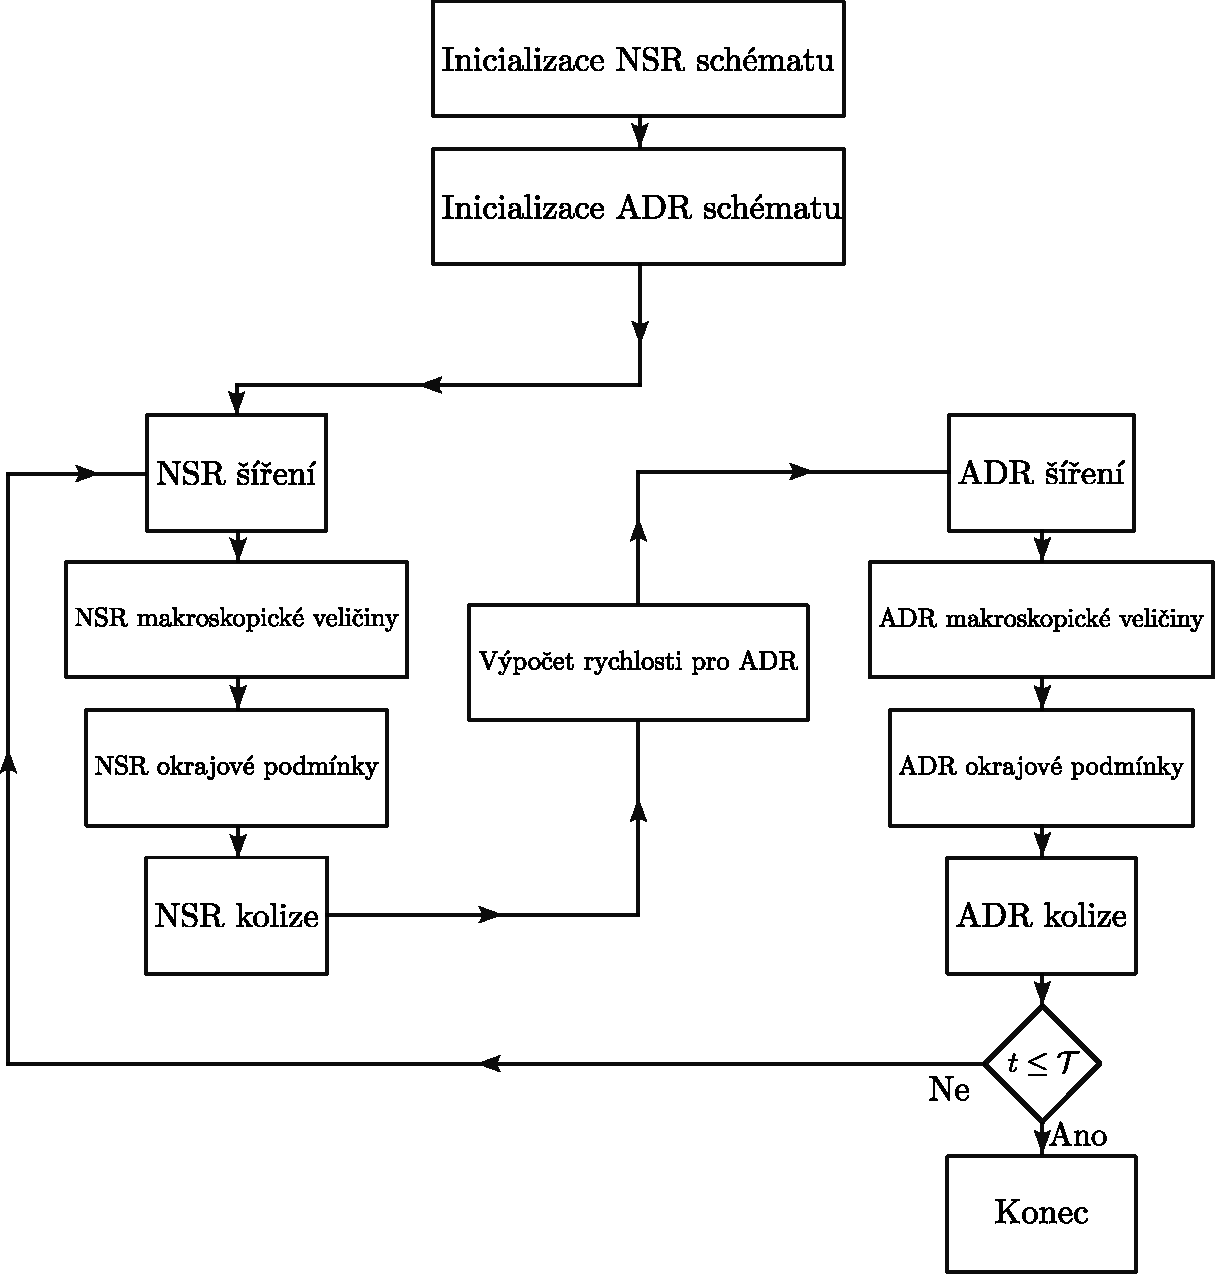
\includegraphics[width=\linewidth]{Img/Kapitola 2/algorithm.pdf}
            \caption{Sch\'{e}ma algoritmu LBM pro \v{r}e\v{s}en\'{\i} NSR a ADR.}
            \label{fig:algorithm}
        \end{figure}   
        

    % % \section{Okrajov\'{e} a po\v{c}\'{a}te\v{c}n\'{\i} podm\'{\i}nky}    
    % % \label{sec:BouIniCon}        
            
    % %     \todo[inline]{P\v{r}epsat} 
    % %     Po\v{c}\'{a}te\v{c}n\'{\i} podm\'{\i}nku 

    % %     P\v{r}i simulaci fyzik\'{a}ln\'{\i} \'{u}lohy m\'{a}me v\v{e}t\v{s}inou zvoleny makroskopick\'{e} parametry \'{u}lohy, jako jsou nap\v{r}\'{\i}klad hustota tekutiny $\rho$, rychlost v oblasti $\boldsymbol{u}$ nebo tlak $p$. Pro tyto parametry je pot\v{r}eba p\v{r}edepsat po\v{c}\'{a}te\v{c}n\'{\i} a okrajov\'{e} podm\'{\i}nky. Jejich formulaci v mezoskopick\'{e}m LBM popisu uvedeme v t\'{e}to kapitole. V\v{s}echny podm\'{\i}nky jsou v t\'{e}to sekci zavedeny pro 2D model. Pro \'{u}plnost zm\'{\i}n\'{\i}me, \v{z}e v p\v{r}\'{\i}pad\v{e} 3D jsou v\v{s}echny podm\'{\i}nky definovan\'{e} analogicky \cite{guo2013lattice, kruger2017lattice}.
        
    % %     \subsection{Po\v{c}\'{a}te\v{c}n\'{\i} podm\'{\i}nka}
    % %     \label{sub:IniCon}
            
    % %         Jednou z mo\v{z}nost\'{\i} na po\v{c}\'{a}te\v{c}n\'{\i} podm\'{\i}nku v \v{c}ase $t=0$ je polo\v{z}it distribu\v{c}n\'{\i} funkce $f_k$ v uzlech $\boldsymbol{x}_{i,j} \in~\hat{\Omega}$  rovny rovnov\'{a}\v{z}n\'{y}m distribu\v{c}n\'{\i}m funkc\'{\i}m $f_{k}^{eq}, \forall k \in \{ 0,1,...,8 \}$, kde $f_{k}^{eq}$ je ur\v{c}eno z p\v{r}edepsan\'{y}ch hodnot hustoty $\rho_{ini}$ a makroskopick\'{e} rychlosti $\boldsymbol{u}_{ini}$, tj. $\forall k \in \{0,1,...,8 \}$ vztahem \eqref{eq:EquDisFun}
            
    % %         % \begin{equation}
    % %         % \label{eq:FirIniCon}
    % %         %     f_k(\boldsymbol{x}_{i,j}, 0) = f_{k}^{eq}(\rho_{ini}(\boldsymbol{x}_{i,j}), \boldsymbol{u}_{ini}(\boldsymbol{x}_{i,j})).
    % %         % \end{equation}
    % %         Tato volba je snadno implementovateln\'{a} a v\'{y}po\v{c}et je m\'{e}n\v{e} \v{c}asov\v{e} n\'{a}ro\v{c}n\'{y}, av\v{s}ak mohou nastat probl\'{e}my s kompatibilitou s okrajov\'{y}mi podm\'{\i}nkami, viz \cite{eichler2018matematicke}.
        
    % %     \subsection{Vstupn\'{\i} podm\'{\i}nka}
    % %     \label{sub:InfCon}
            
    % %         Na vstupn\'{\i} \v{c}\'{a}sti hranice $\hat{\Gamma}_{in}$ p\v{r}edep\'{\i}\v{s}eme hodnoty rovnov\'{a}\v{z}n\'{e} distribu\v{c}n\'{\i} funkce vypo\v{c}\'{\i}tan\'{e} pro~zadanou hustotu a rychlost. V t\'{e}to pr\'{a}ci budeme zkoumat dv\v{e} varianty ($P$ a $G$) tohoto p\v{r}edpisu -- s~konstantn\'{\i} zadanou hustotou ($\rho = 1$) (varianta $P$) a s modifikac\'{\i} odpov\'{\i}daj\'{\i}c\'{\i} p\v{r}edeps\'{a}n\'{\i} gradientu tlaku (varianta $G$). Tuto modifikaci pou\v{z}ijeme pouze ve dvourozm\v{e}rn\'{e} \'{u}loze.
            
    % %         Pro prvn\'{\i} variantu p\v{r}edpokl\'{a}d\'{a}me, \v{z}e do oblasti proud\'{\i} tekutina se zn\'{a}mou hustotou. V LBM je hustota nav\'{a}z\'{a}na na tlak vztahem \eqref{eq:MacPre}, a proto nen\'{\i} tato podm\'{\i}nka konzistentn\'{\i} s okrajovou podm\'{\i}nkou \eqref{eq:DefCasConInl2}.
            
    % %         Ve druh\'{e}m p\v{r}\'{\i}pad\v{e} budeme p\v{r}edpokl\'{a}dat, \v{z}e do oblasti proud\'{\i} tekutina s Hagenov\'{y}m-Poiseullieov\'{y}m rychlostn\'{\i}m profilem a \v{z}e m\'{\i}sto hodnoty tlaku (hustoty) lze na vstupu p\v{r}edepsat hodnotu gradientu tlaku (hustoty) podle vzorce
            
    % %         \begin{equation}
    % %             \frac{\partial p}{\partial x_1} = c_s^2 \frac{\partial \rho}{\partial x_1} = 2 \nu \frac{u_{1}}{\left( \frac{H}{2} \right)^2},
    % %         \end{equation}
    % %         kdy gradient tlaku budeme p\v{r}i samotn\'{e} implementaci aproximovat jeho diferenc\'{\i}.
            
            
            
           
            
            
    %     % \subsection{Periodick\'{a} okrajov\'{a} podm\'{\i}nka}
    %     % \label{sub:PerBouCon}
            
    %     %     P\v{r}i pou\v{z}it\'{\i} t\'{e}to podm\'{\i}nky zajist\'{\i}me periodicitu hranic v oblasti $\Omega$. Uzly na periodick\'{e} \v{c}\'{a}sti hranice se berou jako vnit\v{r}n\'{\i} uzly m\v{r}\'{\i}\v{z}ky a prov\'{a}d\'{\i} se tam kolize podle algoritmu \ref{sec:LbmAlg}. Periodicita se projev\'{\i} a\v{z} p\v{r}i kroku \v{s}\'{\i}\v{r}en\'{\i}. Sch\'{e}ma je pos\'{a}no na obr\'{a}zku \ref{fig:PerBouCon}.
            
    %     %     \begin{figure}[H]
    %     %         \centering
    %     %         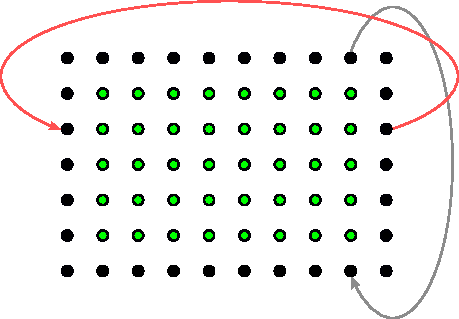
\includegraphics{Img/Kapitola 2/PeriodicBouCon.pdf}
    %     %         \caption{Sch\'{e}ma periodick\'{e} okrajov\'{e} podm\'{\i}nky}
    %     %         \label{fig:PerBouCon}
    %     %     \end{figure}
            
    %     \subsection{Full-way bounce-back okrajov\'{a} podm\'{\i}nka}
    %     \label{sub:BouBacBouCon}
        
    %         Tato okrajov\'{a} podm\'{\i}nka je zalo\v{z}ena na odrazu my\v{s}len\'{y}ch \v{c}\'{a}stic tekutiny od hranice $\hat{\Gamma}$ zp\v{e}t do oblasti s tekutinou $\hat{\Omega}$. D\'{\i}ky t\'{e}to vlastnosti je vhodn\'{a} pro simulace proud\v{e}n\'{\i} tekutiny kolem t\v{e}les. Bylo vyvinuto n\v{e}kolik modifikac\'{\i} t\'{e}to podm\'{\i}nky \cite{kruger2017lattice}. V t\'{e}to pr\'{a}ci zm\'{\i}n\'{\i}me v numerick\'{y}ch simulac\'{\i}ch pou\v{z}itou full-way bounce-back okrajovou podm\'{\i}nku.
            
    %         M\v{e}jme uzel $\boldsymbol{x}_f$ reprezentuj\'{\i}c\'{\i} tekutinu a uzel p\v{r}ek\'{a}\v{z}ky $\boldsymbol{x}_b$ jako na obr\'{a}zku \ref{fig:FulWayBouBac}. V t\'{e}to situaci plat\'{\i} $\boldsymbol{x}_b = \boldsymbol{x}_f + \Delta t \boldsymbol{\xi}_k$ pro index $k \in \{ 4,7,8 \}$, viz \ref{fig:VelMod2a}. Podm\'{\i}nka p\v{r}edepsan\'{a} na hrani\v{c}n\'{\i}ch uzlech se d\'{a} vyj\'{a}d\v{r}it vztahem 
            
    %         \begin{equation}
    %         \label{eq:HalBouBac}
    %             f_{\bar{k}}^*(\boldsymbol{x}_b, t) = f_{k}^{*}(\boldsymbol{x}_f, t - \Delta t) \quad \boldsymbol{x}_b \in \hat{\Gamma}_b, \ \boldsymbol{x}_f \in \hat{\Omega} \backslash \overline{\hat{\Omega}}_b,
    %         \end{equation}
    %         kde pro index $\bar{k}$ plat\'{\i} $\boldsymbol{\xi}_{\bar{k}} = - \boldsymbol{\xi}_{k}$ a $\boldsymbol{x}_b$ je uzel, na kter\'{e}m se p\v{r}edepisuje full-way bounce-back podm\'{\i}nka. D\'{a}le pop\'{\i}\v{s}eme algoritmus pouze pro odraz od bodu $\boldsymbol{x}_b$, pro zb\'{y}vaj\'{\i}c\'{\i} uzly by byl postup analogick\'{y}, viz~obr\'{a}zek \ref{fig:FulWayBouBac}. 
            
    %         P\v{r}i kroku \v{s}\'{\i}\v{r}en\'{\i} v \v{c}ase $t$ je na\v{c}tena hodnota distribu\v{c}n\'{\i} funkce $f_4^*(\boldsymbol{x}_f,t)$ do bod{u} $\boldsymbol{x}_b$. V dal\v{s}\'{\i}m \v{c}ase, nam\'{\i}sto v\'{y}po\v{c}tu kolize, je hodnota funkce $f_4^*(\boldsymbol{x}_f,t)$ zaps\'{a}na do $f_2(\boldsymbol{x}_b,t+\Delta t)$. N\'{a}sledn\v{e} dojde k \v{s}\'{\i}\v{r}en\'{\i} $f_2(\boldsymbol{x}_b,t+\Delta t)$ do uzlu $\boldsymbol{x}_f$.
            
    %         \begin{figure}[ht]
    %             \begin{subfigure}[t]{0.25\textwidth}
    %            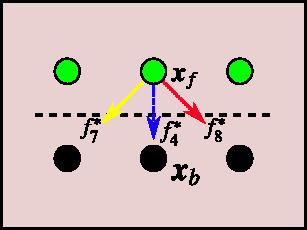
\includegraphics[width=.95\textwidth,valign=t]{Img/Kapitola 2/fullwayBBa.pdf}
    %             \captionof{figure}[t]{Po kolizi v \v{c}ase $t - \Delta t$.}
    %             \label{fig7:FulBouBaca}
    %             \end{subfigure}%
    %             \hfill
    %             %\vspace{2mm}
    %             \begin{subfigure}[t]{0.25\textwidth}
    %            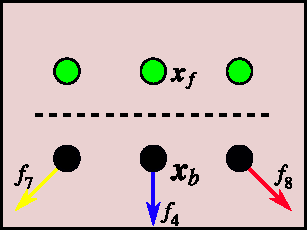
\includegraphics[width=.95\textwidth,valign=t]{Img/Kapitola 2/fullwayBBb.pdf}
    %             \captionof{figure}[t]{Po \v{s}\'{\i}\v{r}en\'{\i} v \v{c}ase $t$.}
    %             \label{fig7:FulBouBacb}
    %             \end{subfigure}%
    %             \hfill
    %             \begin{subfigure}[t]{0.25\textwidth}
    %             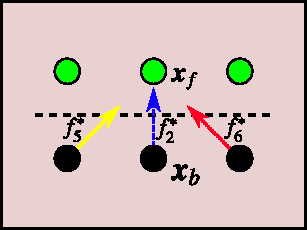
\includegraphics[width=.95\textwidth,valign=t]{Img/Kapitola 2/fullwayBBc.pdf}
    %             \captionof{figure}{Po obr\'{a}cen\'{\i} sm\v{e}ru \\v \v{c}ase $t$.}
    %             \label{fig7:FulBouBacc}
    %             \end{subfigure}%
    %             \hfill
    %             \begin{subfigure}[t]{0.25\textwidth}
               
    %             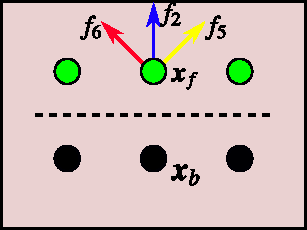
\includegraphics[width=.95\textwidth,valign=t]{Img/Kapitola 2/fullwayBBd.pdf}
    %             \captionof{figure}{Po \v{s}\'{\i}\v{r}en\'{\i} v \v{c}ase $t + \Delta t$.}
    %             \label{fig7:FulBouBacd}
    %             \end{subfigure}
    %             \caption{Sch\'{e}ma full-way bounce-back okrajov\'{e} podm\'{\i}nky na rozhran\'{\i} mezi $\boldsymbol{x}_f$ a $\boldsymbol{x}_b$.}
    %             \label{fig:FulWayBouBac}
    %         \end{figure}
        
    %     \subsection{Odtokov\'{a} okrajov\'{a} podm\'{\i}nka}
    %     \label{sub:OutBouCon}
        
    %         Na \v{c}\'{a}sti hranice $\hat{\Gamma}_{out}$ nastav\'{\i}me odtokovou podm\'{\i}nku dle \cite{geier2015cumulant}. Pro hrani\v{c}n\'{\i} uzly p\v{r}\'{\i}slu\v{s}ej\'{\i}c\'{\i} $\Gamma_{out}$ neexistuje uzel, od kter\'{e}ho by obdr\v{z}ely hodnotu distribu\v{c}n\'{\i}ch funkc\'{\i} ve sm\v{e}rech $\boldsymbol{\xi}_k, k \in \{ 3, 6, 7 \}$. \v{R}e\v{s}en\'{\i}m je nastavit p\v{r}i kroku \v{s}\'{\i}\v{r}en\'{\i} hodnotu t\v{e}chto distribu\v{c}n\'{\i}ch funkc\'{\i} dle vztahu
            
    %         \begin{equation}
    %         \label{eq:GraDisFunTimNorVec}
    %             \nabla f_k \cdot \boldsymbol{n} = 0 \quad \forall k \in \{ 3,6,7 \},
    %         \end{equation}
    %         tj. zkop\'{\i}rujeme hodnoty dan\'{y}ch distribu\v{c}n\'{\i}ch funkc\'{\i} z uzlu p\v{r}ede\v{s}l\'{e}ho (ve sm\v{e}ru od hranice dovnit\v{r} oblasti), viz obr\'{a}zek \ref{fig:Out}. V rovnici vystupuje norm\'{a}lov\'{y} vektor $\boldsymbol{n}$ ve sm\v{e}ru vn\v{e}j\v{s}\'{\i} norm\'{a}ly k hranici $\hat{\Gamma}_{out}$.
            
    %         \begin{figure}[H]
    %             \centering
    %             \begin{subfigure}{.5\textwidth}                        
    %                 \centering
    %                 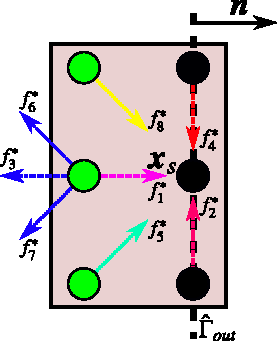
\includegraphics[width=.485\textwidth]{Img/Kapitola 2/outflowaa.pdf} \captionof{figure}{P\v{r}ed \v{s}\'{\i}\v{r}en\'{\i}m v \v{c}ase $t$.}
    %                 \label{fig:Outa}
    %             \end{subfigure}%
    %              \begin{subfigure}{.5\textwidth}                        
    %                 \centering
    %                 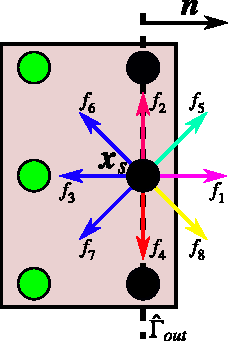
\includegraphics[width=.4\textwidth]{Img/Kapitola 2/outflowbb.pdf} \captionof{figure}{Po \v{s}\'{\i}\v{r}en\'{\i} v \v{c}ase $t + \Delta t$.}
    %               \label{fig:Outb}
    %             \end{subfigure}%
    %             \caption{Sch\'{e}ma definice postkolizn\'{\i}ch distribu\v{c}n\'{\i}ch funkc\'{\i} p\v{r}i odtokov\'{e} okrajov\'{e} podm\'{\i}nce, kter\'{e}~budou pou\v{z}ity p\v{r}i kolizn\'{\i}m kroku v uzlu $\boldsymbol{x}_s$ v \v{c}ase $t +\Delta t$. P\v{r}eru\v{s}ovan\'{e} \v{s}ipky zna\v{c}\'{\i} postkolizn\'{\i} distribu\v{c}n\'{\i} funkce, pln\'{e} reprezentuj\'{\i} distribu\v{c}n\'{\i} funkce, kter\'{e} jsou po kroku \v{s}\'{\i}\v{r}en\'{\i}. Na \v{c}\'{a}rkovan\'{e} hranici $\Gamma_{out}$ je vyzna\v{c}en vn\v{e}j\v{s}\'{\i} norm\'{a}lov\'{y} vektor $\boldsymbol{n}$.}    
    %             \label{fig:Out}
    %         \end{figure}

        % \section{Momentov\'{e} okrajov\'{e} podm\'{\i}nky}
        % \todo[inline]{Doplnit?? Vymyslet \'{u}lohu, na kter\'{e} testovat star\'{e} OP a momentov\'{e} - jinak nepsat}


            % Relaxa\v{c}n\'{\i} \v{c}asy vol\'{\i}me za p\v{r}edpokladu izotropn\'{\i} viskozity n\'{a}sledovn\v{e}
            
            % \begin{subequations}
            % \begin{align}
            %     \tau_4 = \tau_5& = \tau_{shear}, \\
            %     \tau_3 = \tau_6 = \tau_7& = \tau_8 = 1,
            % \end{align}
            % \end{subequations}
            % kde \v{c}asy $\tau_3, \tau_6, \tau_7, \tau_8$ jsou voleny ke zlep\v{s}en\'{\i} numerick\'{e} stability kolizn\'{\i}ho modelu CLBM a vztah mezi~viskozitou a relaxa\v{c}n\'{\i}m \v{c}asem $\tau_{shear}$ je stejn\'{y} jako u jin\'{y}ch kolizn\'{\i}ch model\r{u} \cite{geier2015cumulant}, tj.
            
            % \begin{equation}
            % \label{eq:ClbVis}
            %     \nu_{LBM} = c_s^2 \left( \tau_{shear} - \frac{\Delta t}{2} \right).
            % \end{equation}
            
            % Pro implementaci je pou\v{z}ita kask\'{a}dov\'{a} varianta CLBM \cite{geier2007properties}, kde ni\v{z}\v{s}\'{\i} momenty slou\v{z}\'{\i} k v\'{y}po\v{c}tu moment\r{u} vy\v{s}\v{s}\'{\i}ch.
            

            


        % \subsection{CuLBM}
        % \label{sub:CuLBM}
            
        %     Sch\'{e}ma LBM \v{r}e\v{s}\'{\i}c\'{\i} Navierovy-Stokesovy rovnice pro proud\v{e}n\'{\i} je dopln\v{e}no o Kumulantn\'{\i} LBM kolizn\'{\i} oper\'{a}tor (CuLBM). Prvn\'{\i} zm\'{\i}nka o tomto oper\'{a}toru poch\'{a}zi z roku 2015 \cite{geier2015cumulant}. 

        %     Z\'{a}kladem oper\'{a}toru jsou relaxa\v{c}n\'{\i} \v{c}asy makroskopick\'{y}ch moment\r{u}, kter\'{e} jsou z\'{a}rove\v{n}  Galileovsky invariantn\'{\i}  statisticky nez\'{a}visl\'{e}.

        %     M\v{e}jme nyn\'{\i} rychlostn\'{\i} model $D3Q27$ a podobn\v{e} jako u CLBM vyu\v{z}ijeme obedn\'{y}ch a centr\'{a}ln\'{\i}ch moment\r{u}
        %     \begin{equation}
        %     \label{eq:RawMomCum}
        %         m_{\boldsymbol{\boldsymbol{\alpha}}} \coloneqq \sum_{k=0}^{26}f_k \xi_{k,1}^{\alpha_1}{\xi}_{k,2}^{\alpha_2}{\xi}_{k,3}^{\alpha_3},
        %     \end{equation}
        %     a
        %     \begin{equation}
        %     \label{eq:CenMomCum}
        %         k_{\boldsymbol{\boldsymbol{\alpha}}} \coloneqq \sum_{k=0}^{26}f_k ({\xi}_{k,1} - {u}_{1})^{\alpha_1}({\xi}_{k,2} - {u}_{2})^{\alpha_2}({\xi}_{k,3} - {u}_{3})^{\alpha_3}. 
        %     \end{equation}
        %     kde $\boldsymbol{\alpha}$ a $\boldsymbol{u}$ zna\v{c}\'{\i} stejn\v{e} jako v sekci \ref{sub:CLBM} multiindex a makroskopickou rychlost.

        %     Tentokr\'{a}t m\'{a}me kolizn\'{\i} oper\'{a}tor ve tvaru
        %     \begin{equation}
        %         \label{eq:CumOpe}
        %             \mathcal{C}(\boldsymbol{f}(\boldsymbol{x},t)) = \boldsymbol{M}^{-1}\boldsymbol{G}^{-1}\left(\boldsymbol{N}^{-1}\boldsymbol{S}\boldsymbol{N}\boldsymbol{G}\Big(\boldsymbol{M}\boldsymbol{f}^{eq}(\boldsymbol{x},t) - \boldsymbol{M}\boldsymbol{f}(\boldsymbol{x},t)\Big)\right),
        %     \end{equation}
        %     tud\'{\i}\v{z} pro postkolizn\'{\i} distribu\v{c}n\'{\i} funkci dost\'{a}v\'{a}me vztah
        %     \begin{equation}
        %     \label{eq:PosColCum}
        %         \boldsymbol{f}^{*}(\boldsymbol{x},t) = \boldsymbol{f}(\boldsymbol{x},t) + \boldsymbol{M}^{-1}\boldsymbol{G}^{-1}\left(\boldsymbol{N}^{-1}\boldsymbol{S}\boldsymbol{N}\boldsymbol{G}\Big(\boldsymbol{M}\boldsymbol{f}^{eq}(\boldsymbol{x},t) - \boldsymbol{M}\boldsymbol{f}(\boldsymbol{x},t)\Big)\right),
        %     \end{equation}
        %     kde matice $\boldsymbol{S}$ je pro relaxa\v{c}n\'{\i} \v{c}asy $\tau_i, i \in \{ 0,1,...,26 \}$ ve tvaru
        %     \begin{equation}
        %     \label{eq:MatSCum}
        %         \boldsymbol{S} = \mathrm{diag}\Bigg(0, 0, 0, 0,  \frac{\Delta t}{\tau_1}, \frac{\Delta t}{\tau_2}, \frac{\Delta t}{\tau_3}, \frac{\Delta t}{\tau_4},...,\frac{\Delta t}{\tau_{22}}, \frac{\Delta t}{\tau_{23}} \Bigg).
        %     \end{equation}
        %     Pomoc\'{\i} matice $\boldsymbol{M}$ definujeme vektor makroskopick\'{y}ch moment\r{u} $\boldsymbol{\mu}$ jako
        %     \begin{equation}
        %         \label{eq:MatMCum}    
        %             \boldsymbol{\mu} = \boldsymbol{M}\boldsymbol{f}.
        %     \end{equation}
        %     Dal\v{s}\'{\i} matic\'{\i}, kter\'{a} vystupuje ve vztahu \eqref{eq:PosColCum}, je matice kombinace kumulant\r{u} $\boldsymbol{N}$. Podrobn\'{y} popis t\v{e}chto matic lze nal\'{e}zt v \cite{geier2015cumulant}. Posledn\'{\i}m v\'{y}razem, kter\'{y} vystupuje ve vztahu pro postkolizn\'{\i} funkce, je neline\'{a}rn\'{\i} oper\'{a}tor $\boldsymbol{G}$, za pomoci kter\'{e}ho je provedena transformace obecn\'{y}ch moment\r{u} $\boldsymbol{\mu}$ do kumulantn\'{\i}ho vektoru  
        %     \begin{equation}
        %         \label{eq:OpeGCum}
        %             \boldsymbol{\gamma} = \boldsymbol{G}(\boldsymbol{\mu}) = \boldsymbol{G(Mf)} = \left( \gamma_{(0,0,0)}, \gamma_{(1,0,0)}, \gamma_{(0,1,0)},..., \gamma_{(2,2,2)} \right)^T.
        %     \end{equation}
        %     Nakonec definujeme vektor 
        %     \begin{equation}
        %         \label{eq:GamEquCum}
        %             \boldsymbol{\gamma}^{eq} = \left( \rho, 0, 0, 0, 0, 0, 0, 0, 0, 3\rho c_s^2, 0, 0,...,0 \right)^T 
        %     \end{equation}
        %     a n\'{a}sledn\v{e} m\r{u}\v{z}eme vztah \eqref{eq:PosColCum} p\v{r}epsat v \v{r}e\v{c}i vektoru $\boldsymbol{\gamma}$
        %     \begin{equation}
        %         \label{eq:PosColCumGam}
        %             \boldsymbol{\gamma}^* (\boldsymbol{x},t) = \boldsymbol{\gamma} (\boldsymbol{x},t) + \boldsymbol{N}^{-1}\boldsymbol{S}\boldsymbol{N} \Big( \boldsymbol{\gamma}^{eq} (\boldsymbol{x},t) - \boldsymbol{\gamma} (\boldsymbol{x},t)\Big).
        %     \end{equation}

        %     P\v{r}edpokl\'{a}d\'{a}me-li izotropn\'{\i} viskozitu, lze volit relaxa\v{c}n\'{\i} \v{c}asy 
        %     \begin{subequations}
        %         \begin{align}
        %             \tau_1 &= \tau_{shear}, \\
        %             \tau_i &= 1  \qquad \forall i \in \{ 2,3,4,...23 \}, 
        %         \end{align}
        %     \end{subequations}
        %     kde $\tau_{shear}$ spl\v{n}uje
        %     \begin{equation}
        %         \nu_{LBM} = c_s^2 \left( \tau_{shear} - \frac{\Delta t}{2} \right).
        %     \end{equation}



% \subsection{SRT}
        % \label{sub:Srt}
        
        %     Kolizn\'{\i} oper\'{a}tor SRT (Single Relaxation Time, tedy LBM s jedn\'{\i}m relaxa\v{c}n\'{\i}m \v{c}asem) \cite{eichler2016matematicke} je nejjednodu\v{s}\v{s}\'{\i}m ze v\v{s}ech oper\'{a}tor\r{u}. P\r{u}vod m\'{a} u Bhatnagarova-Grossova-Krookova (BGK) kolizn\'{\i}ho modelu \v{c}\'{a}stic \cite{eichler2016matematicke} a lze jej aproximovat ve tvaru
            
        %     \begin{equation}
        %     \label{eq:SrtOpe}
        %         C_{k}^{SRT}(\boldsymbol{x}, t) = -\frac{\Delta t}{\tau} ( f_k(\boldsymbol{x}, t) - f_{k}^{eq}(\boldsymbol{x}, t)) \qquad \forall \boldsymbol{x} \in \hat{\Omega}, \forall t \in \hat{\mathcal{I}}, 
        %     \end{equation}
        %     kde relaxa\v{c}n\'{\i} \v{c}as $\tau$ zna\v{c}\'{\i}, jak rychle syst\'{e}m sm\v{e}\v{r}uje do lok\'{a}ln\'{\i} rovnov\'{a}hy ur\v{c}en\'{e} $f_{k}^{eq}$, $k \in \{ 0,1,...,q-1 \}$. Lok\'{a}ln\'{\i} rovnov\'{a}ha je stav, kdy se lok\'{a}ln\'{\i} veli\v{c}iny v \v{c}ase nem\v{e}n\'{\i}. Parametr $\tau$ je ur\v{c}en viskozitou vztahem \cite{kruger2017lattice}
            
        %     \begin{equation}
        %     \label{eq:KinVis}
        %         \nu_{LBM} = c_{s}^{2} \left( \tau - \frac{\Delta t}{2} \right).
        %     \end{equation}
    
              
    
%     \section{Pozn\'{a}mky k implementaci}            
        
%         V t\'{e}to sekci pop\'{\i}\v{s}eme implementaci v\'{y}po\v{c}tu s\'{\i}ly metodou v\'{y}m\v{e}ny hybnosti, kter\'{y} byl form\'{a}ln\v{e} pops\'{a}n v sekci \ref{sec:MomExcMet}.
        
%         Uva\v{z}ujme 2D \'{u}lohu \ref{sec:DefCas2D} s kruhovou p\v{r}ek\'{a}\v{z}kou se st\v{r}edem v bod\v{e} \texttt{\lstinline{(sx,sy)}} o polom\v{e}ru \texttt{\lstinline{r-1}}. Pro~v\'{y}po\v{c}et celkov\'{e} s\'{\i}ly \texttt{\lstinline{(Fx,Fy)}}, kterou p\v{r}ek\'{a}\v{z}ka p\r{u}sob\'{\i} na tekutinu, budeme proch\'{a}zet jednotliv\'{e} uzly tekutiny soused\'{\i}c\'{\i} s p\v{r}ek\'{a}\v{z}kou za pomoci  \texttt{\lstinline{bool wall}}: 
        
%         \begin{lstlisting}[frame=single, backgroundcolor=\color{light-gray}, commentstyle=\color{codegray}, basicstyle=\footnotesize\ttfamily, language=C++, numbers=left, numberstyle=\tiny\color{black}]
% Fx = 0;
% Fy = 0;
% // scanning neighborhood of the obstacle
% for( int x = sx-r; x <= sx+r; x++ )
% {
%     for( int y = sy-r; y <= sy+r; y++ )
%     {
%         if( map( x,y ) == LBM_BC::GEO_FLUID )
%         {
%             // scanning for neighboring wall nodes
%       	    bool wall = false;
%     	    for( int i = -1; i <= 1; i++ )
%     		for( int j = -1; j <= 1 ; j++ )
%                     if( map( x+i,y+j ) == LBM_BC::GEO_WALL )
%                         wall = true;
%     	    // if the neighboring node is a wall, its contribution is computed
%     	    if ( wall ) 
%             {
%                 real fx, fy;
%                 ComputeForce( x,y,fx,fy );
%                 Fx += fx;
%                 Fy += fy;	
%             }
%         }
%     }
% }			    
%         \end{lstlisting}
%     \clearpage
%         V p\v{r}\'{\i}pad\v{e}, \v{z}e dan\'{y} uzel s p\v{r}ek\'{a}\v{z}kou soused\'{\i}, vypo\v{c}teme pro tento uzel p\v{r}\'{\i}sp\v{e}vek k celkov\'{e} s\'{\i}le \texttt{\lstinline{(fx,fy)}} pomoc\'{\i} funkce \texttt{\lstinline{ComputeForce()}}:

%         \begin{lstlisting}[frame=single, backgroundcolor=\color{light-gray}, commentstyle=\color{codegray}, basicstyle=\footnotesize\ttfamily, language=C++, numbers=left, numberstyle=\tiny\color{black}, escapechar=\%]
% void ComputeForce( int x,int y,real &fx,real &fy )
% {
%     // array used for computing contribution to this node's force
%     dreal SS[ 8 ];
%     // array used for setting weights
%     dreal W[ 8 ];
    
%     // set scalar array W  
%     for( int i = 0; i <= 7; i++ )
%         W[ i ] = 1;
%     if( map( x-1,y ) == LBM_BC::GEO_WALL )
%         W[ mz ] = 0;
%     if( map( x,y-1 ) == LBM_BC::GEO_WALL )
%         W[ zm ] = 0;
%     if( map( x+1,y ) == LBM_BC::GEO_WALL )
%         W[ pz ] = 0;
%     if( map( x,y+1 ) == LBM_BC::GEO_WALL )
%         W[ zp ] = 0;
%     if( map( x-1,y-1 ) == LBM_BC::GEO_WALL )
%         W[ mm ] = 0;
%     if( map( x+1,y-1 ) == LBM_BC::GEO_WALL )
%         W[ pm ] = 0;
%     if( map( x+1,y+1 ) == LBM_BC::GEO_WALL )
%         W[ pp ] = 0;
%     if( map( x-1,y+1 ) == LBM_BC::GEO_WALL )
%         W[ mp ] = 0;
    
%     // compute momentum exchange according to the equation %\eqref{eq:MomExc}%
%     SS[ pz ] = ( pdf[ Fxy(pz,x,y,X,Y) ] + pdf[ Fxy(mz,x-1,y,X,Y) ] ) * W[ mz ];
%     SS[ zp ] = ( pdf[ Fxy(zp,x,y,X,Y) ] + pdf[ Fxy(zm,x,y-1,X,Y) ] ) * W[ zm ];
%     SS[ mz ] = ( pdf[ Fxy(mz,x,y,X,Y) ] + pdf[ Fxy(pz,x+1,y,X,Y) ] ) * W[ pz ];
%     SS[ zm ] = ( pdf[ Fxy(zm,x,y,X,Y) ] + pdf[ Fxy(zp,x,y+1,X,Y) ] ) * W[ zp ];
%     SS[ pp ] = ( pdf[ Fxy(pp,x,y,X,Y) ] + pdf[ Fxy(mm,x-1,y-1,X,Y) ] ) * W[ mm ];
%     SS[ mp ] = ( pdf[ Fxy(mp,x,y,X,Y) ] + pdf[ Fxy(pm,x+1,y-1,X,Y) ] ) * W[ pm ];
%     SS[ mm ] = ( pdf[ Fxy(mm,x,y,X,Y) ] + pdf[ Fxy(pp,x+1,y+1,X,Y) ] ) * W[ pp ];
%     SS[ pm ] = ( pdf[ Fxy(pm,x,y,X,Y) ] + pdf[ Fxy(mp,x-1,y+1,X,Y) ] ) * W[ mp ];
    
%     // node contribution to the total force     
%     fx = SS[ pp ] + SS[ pz ] + SS[ pm ] - SS[ mm ] - SS[ mz ] - SS[ mp ];
%     fy = SS[ pp ] + SS[ zp ] + SS[ mp ] - SS[ pm ] - SS[ mm ] - SS[ zm ];
% }			    
%         \end{lstlisting}
%         Tato funkce nejprve nastav\'{\i} hodnoty pro pole \texttt{\lstinline{W}} -- nulov\'{a} bude v p\v{r}\'{\i}pad\v{e}, \v{z}e se v dan\'{e}m sm\v{e}ru nach\'{a}z\'{\i} uzel p\v{r}ek\'{a}\v{z}ky, v opa\v{c}n\'{e}m p\v{r}\'{\i}pad\v{e} je hodnota nastavena na 1. Pozice dan\'{e}ho sm\v{e}ru v poli je dan\'{a} indexy \texttt{\lstinline{ij}}, kde \texttt{\lstinline{i,j}} $\in \texttt{\{\lstinline{m, z, p}\}}$ (p\'{\i}smena zna\v{c}\'{\i} zm\v{e}nu pozice na dan\'{e} sou\v{r}adnici -- "\texttt{\lstinline{m}}" \ odpov\'{\i}d\'{a} hodnot\v{e} -1, "\texttt{\lstinline{p}}" \ zna\v{c}\'{\i} hodnotu +1 a v p\v{r}\'{\i}pad\v{e} "\texttt{\lstinline{z}}" \ se hodnota nem\v{e}n\'{\i}).
        
%         Po nastaven\'{\i} pole \texttt{\lstinline{W}} se spo\v{c}\'{\i}taj\'{\i} p\v{r}\'{\i}sp\v{e}vky od jednotliv\'{y}ch sm\v{e}r\r{u} \texttt{\lstinline{SS[ ij ]}}, pro \texttt{\lstinline{i,j}} $\in \texttt{\{\lstinline{m, z, p}\}}$  za pomoci distribu\v{c}n\'{\i}ch funkc\'{\i} \texttt{\lstinline{pdf[]}} z\'{\i}skan\'{y}ch po kroku \v{s}\'{\i}\v{r}en\'{\i} dle vztahu \eqref{eq:MomExc}. Nakonec jsou jednotliv\'{e} p\v{r}\'{\i}sp\v{e}vky nas\v{c}\'{\i}t\'{a}ny do \texttt{\lstinline{(fx,fy)}}, \v{c}\'{\i}m\v{z} z\'{\i}sk\'{a}me p\v{r}\'{\i}sp\v{e}vek dan\'{e}ho uzlu k celkov\'{e} s\'{\i}le po\v{c}\'{\i}tan\'{e} vztahem \eqref{eq:ForMomExc}.